\section{Examples for a 3D Subduction Zone}
\label{sec:example:subduction:3d}

% ----------------------------------------------------------------------
\subsection{Overview}

This suite of examples demonstrates use of a wide variety of features
and the general workflow often used in research simulations. We base
the model on the Cascadia subduction zone
(Figure~\vref{fig:example:subduction:3d:cascadia}). These examples will
focus on modeling the deformation associated with the the subducting
slab, including interseismic deformation with aseismic slip (creep)
and viscoelastic relaxation, coseismic slip on the slab interface and
a splay fault, and slow slip events on the top slab interface. We want
to account for the 3-D material properties associated with different
elastic properties for the subducting slab, mantle, continental crust,
and an accretionary wedge. To keep the computation time in these
examples short, we limit our model to an 800 km $\times$ 800 km
$\times$ 400 km domain and we will use a relatively coarse
discretization. For simplicity and to reduce complexity in constructing
the mesh, we use a flat top surface (elevation of 0 with respect
to mean sea level).

\begin{figure}[htbp]
  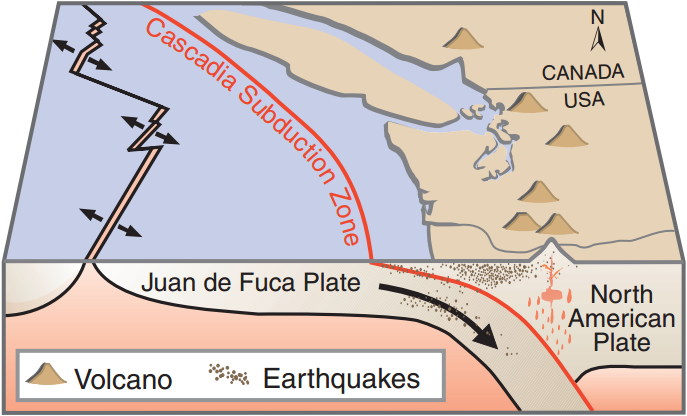
\includegraphics[width=4.5in]{examples/figs/subduction3d_cascadia}
  \caption{Cartoon of the Cascadia Subduction Zone showing the
    subduction of the Juan de Fuca Plate under the North American
    Plate. Source:
    \href{https://pubs.usgs.gov/fs/2000/fs060-00/}{U.S. Geological
      Survey Fact Sheet 060-00}}
  \label{fig:example:subduction:3d:cascadia}
\end{figure}

Figure~\vref{fig:example:subduction:3d:concept} shows our conceptual
model with a slab, mantle, continental crust, and accretionary
wedge. We cut off the slab at a depth of 100 km. We use a transverse
geographic projection coordinate system with Portland, Oregon, as the
origin in order to georeference our model. In order to model the
motion of the slab, we include a fault on the top of the slab at the
interface between the mantle, crust, and wedge, as well as a fault
between the bottom of the slab and the mantle.

\begin{figure}[htbp]
  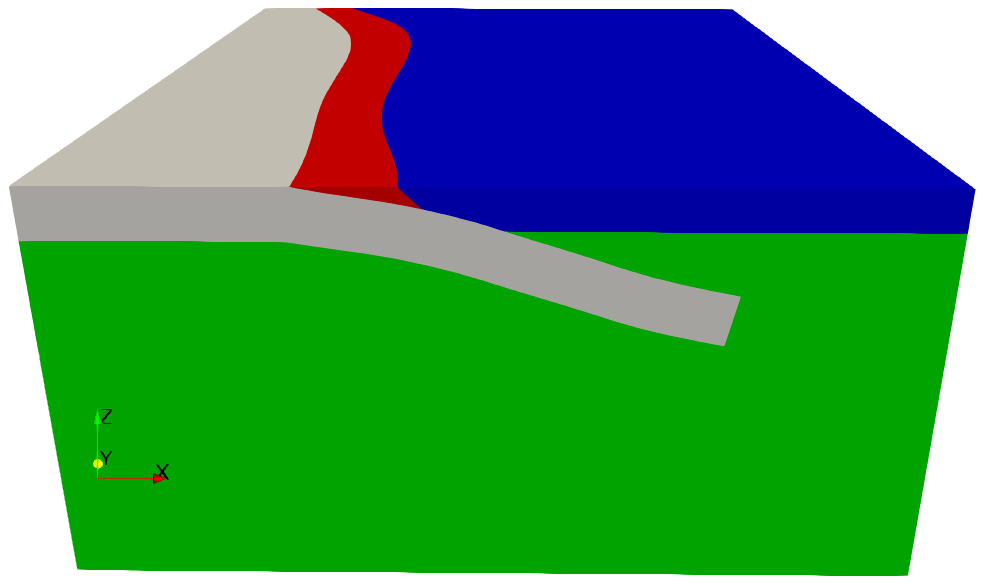
\includegraphics[width=4.5in]{examples/figs/subduction3d_conceptualmodel}
  \caption{Conceptual model based on the Cascadia Subduction Zone. The
    model includes the subduction slab (white), the mantle (green),
    continental crust (blue), and an acrretionary wedge (red).}
  \label{fig:example:subduction:3d:concept}
\end{figure}

The files associated with this suite of examples are contained in the
directory \filename{examples/3d/subduction}. This directory contains
several subdirectories:
\begin{description}
\item[\filename{mesh}] Files used to construct the finite-element mesh using
  CUBIT/Trelis.
\item[\filename{spatialdb}] Files associated with the spatial
  and temporal databases.
\item[\filename{viz}] ParaView
  Python scripts and other files for visualizing results.
\item[\filename{output}] Directory containing simulation
  output. It is created automatically when running the
  simulations.
\end{description}


% ----------------------------------------------------------------------
\subsection{Features Illustrated}

Table~\vref{tab:example:subduction:3d:features} lists the features
discussed in each of these 3-D subduction zone examples. With the
intent of illustrating features used in research simulations, we use
HDF5 output and, we make extensive use the most efficient
implementations of spatial databases (UniformDB and SimpleGridDB). We
also use ParaView Python scripts for visualizing the output. These
scripts can be run within the ParaView GUI or outside the ParaView
GUI, although the interaction is limited to rotating, translating, and
zooming when run outside the ParaView GUI.

\todo{brad}{Complete filling in table.}
\begin{table}[htbp]
  \caption{PyLith features covered in the suite of 3-D subduction zone examples.}
  \label{tab:example:subduction:3d:features}
  \rowcolors{2}{yellow!30}{white}
\resizebox{\textwidth}{!}{%
\begin{tabular}{|l|%% Example
    *{8}c|% General
    *{3}c|% Solver
    *{5}c|% Spatial Database
}
\hline
\rowcolor{blue!10}
Example
& \multicolumn{8}{c|}{General}
& \multicolumn{3}{c|}{Solver}
& \multicolumn{5}{c|}{Spatial Database}
\\ 
%%%%
\hline
\rowcolor{blue!10}

% General
& \rlabel{Dimension}
& \rlabel{Coordinate system}
& \rlabel{Mesh generator}
& \rlabel{Cells}
& \rlabel{Refinement}
& \rlabel{Reordering}
& \rlabel{Problem type}
& \rlabel{Time dependence}
% Solver
& \rlabel{Solver}
& \rlabel{Preconditioner}
& \rlabel{Time stepping}
% Spatial Database
& \rlabel{Uniform}
& \rlabel{Simple}
& \rlabel{Simple grid}
& \rlabel{Composite}
& \rlabel{Time history}
\\
\hline
3d/subduction/step01
& 3 & Proj & CUBIT & Tet & & \yes & TD & S 
& L & ILU & 
& x2 & x4 & & & 
\\ \hline
3d/subduction/step02
& 3 & Proj & CUBIT & Tet & & \yes & TD & QS 
& L & ML+CUST & BE 
& x2 & x3 & x2 & x2 & 
\\ \hline
3d/subduction/step03
& 3 & Proj & CUBIT & Tet & & \yes & TD & QS 
& L & ML+CUST & BE 
& x4 & x3 & x2 & x2 & 
\\ \hline
3d/subduction/step04
& 3 & Proj & CUBIT & Tet & & \yes & TD & QS 
& L & ML+CUST & BE 
& x7 & x3 & x5 & x2 & 
\\ \hline
3d/subduction/step05
& 3 & Proj & CUBIT & Tet & & \yes & TD & QS 
& NL & ML+CUST & BE 
& x7 & x3 & x5 & x2 & 
\\ \hline
3d/subduction/step06
& 3 & Proj & CUBIT & Tet & & \yes & TD & QS 
& NL & ML+CUST & BE 
& x1 & x4 & x1 & & x1 
\\ \hline
\end{tabular}}
\par
{\bf Problem type} -- TD: time dependent, GF: Green's functions. {\bf Time dependence} -- S: static, QS: quasi-static, D: dynamic. {\bf Solver} -- L: linear, NL: nonlinear. {\bf Preconditioner} -- ILU: ILU, ASM: Additive Schwarz, SCHUR: Schur complement, CUST: custom, ML: ML algebraic multigrid, GAMG: geometric algebraic multigrid. {\bf Time stepping} -- BE: Backward Euler, FE: Forward Euler. \\ 
\rowcolors{2}{yellow!30}{white}
\resizebox{\textwidth}{!}{%
\begin{tabular}{|l|%% Example
    *{4}c|% Boundary Condition
    *{8}c|% Fault
    *{9}c|% Bulk Rheology
    *{7}c|% Output
}
\hline
\rowcolor{blue!10}
Example
& \multicolumn{4}{c|}{Boundary Condition}
& \multicolumn{8}{c|}{Fault}
& \multicolumn{9}{c|}{Bulk Rheology}
& \multicolumn{7}{c|}{Output}
\\ 
%%%%
\hline
\rowcolor{blue!10}

% Boundary Condition
& \rlabel{Dirichlet}
& \rlabel{Neumann}
& \rlabel{Absorbing}
& \rlabel{Point force}
% Fault
& \rlabel{Prescribed slip}
& \rlabel{Slip time function}
& \rlabel{Constitutive model}
& \rlabel{Static friction}
& \rlabel{Slip-weakening friction}
& \rlabel{Time-weakening friction}
& \rlabel{Rate-state friction w/ageing}
& \rlabel{Traction perturbation}
% Bulk Rheology
& \rlabel{Linear elastic}
& \rlabel{Linear Maxwell viscoelastic}
& \rlabel{Generalized Maxwell viscoelastic}
& \rlabel{Powerlaw viscoelastic}
& \rlabel{Drucker-Prager elastoplastic}
& \rlabel{Stress/strain formulation}
& \rlabel{Inertia}
& \rlabel{Reference state}
& \rlabel{Gravity}
% Output
& \rlabel{Format}
& \rlabel{Domain output}
& \rlabel{Surface output}
& \rlabel{Point output}
& \rlabel{State variable output}
& \rlabel{ParaView}
& \rlabel{Matplotlib}
\\
\hline
3d/subduction/step01
& x5 & & & 
& & & & & & & & & x4 & & & & & Inf & & & 
& H5 & x1 & x1 & & x4 & \yes & 
\\ \hline
3d/subduction/step02
& x5 & & & 
& x1 & STEP & & & & & & 
& x2 & x2 & & & & Inf & & & 
& H5 & x1 & x1 & & x4 & \yes & 
\\ \hline
3d/subduction/step03
& x5 & & & 
& x2 & RATE & & & & & & 
& x2 & x2 & & & & Inf & & & 
& H5 & x1 & x1 & & x4 & \yes & 
\\ \hline
3d/subduction/step04
& x5 & & & 
& x3 & STEP & & & & & & 
& x2 & x2 & & & & Inf & & & 
& H5 & x1 & x1 & & x4 & \yes & 
\\ \hline
3d/subduction/step05
& x5 & & & 
& x1 & RATE & x1 & & \yes & & & \yes 
& x2 & x2 & & & & Inf & & & 
& H5 & x1 & x1 & & x4 & \yes & 
\\ \hline
3d/subduction/step06
& x5 & & & 
& x1 & USER & & & & & & 
& x4 & & & & & Inf & & & 
& H5 & x1 & x1 & x1 & x4 & \yes & 
\\ \hline
\end{tabular}}
\par
{\bf Stress/strain formulation} -- Inf: infinitesimal, Fin: small, finite strain. \\ 

\end{table}

% ----------------------------------------------------------------------
\subsection{Generating the Finite-Element Mesh}

We use CUBIT/Trelis to generate the finite-element mesh. Due to its
size, we do not include the finite-element mesh in the PyLith source
or binary distributions. If you do not have CUBIT/Trelis, you can
download the mesh from
\url{https://wiki.geodynamics.org/software:pylith:examples:files} and
skip generating the mesh.

We use contours of the Cascadia Subduction Zone from Slab v1.0
\cite{Hayes:etal:2012} for the geometry of the top of the slab. In
order to make use of these contours from within CUBIT/Trelis, we use a
Python script (\filename{generate\_surfjou.py}) to read the contours
file and create a CUBIT/Trelis journal file
(\filename{generate\_surfs.jou}) that adds additional contours west of
the trench and then constructs the top and bottom surfaces of the
slab. The Python script also constructs a splay fault by copying a
contour to a depth below the slab and above the ground surface.

\tip{We define the coordinate systems we use in the simulations in the
  the Python script \filename{coordsys.py} to make it easier to
  convert to/from various georeference coordinate systems in the pre-
  and post-processing. PyLith will automatically convert among
  compatible coordinate systems during the simulation.}

\begin{shell}
# Make sure you are in the 'mesh' directory and then run the Python
# script to generate the journal file 'generate_surfs.jou'.
$$ ./generate_surfjou.py  
\end{shell}

The next step is to use CUBIT/Trelis to run the
\filename{generate\_surfs.jou} journal file to generate the spline
surfaces for the slab and splay fault and save them as ACIS
surfaces. 

\important{The CUBIT/Trelis journal files name objects and then later
  reference them by name. When objects are cut, a suffix of
  \object{@LETTER} is appended to the original name (for example,
  \object{domain} becomes \object{domain} and
  \object{domain@A}). However, which one retains the original name and
  which ones gets the suffix is ambiguous. In general, the names are
  consistent across versions of CUBIT/Trelis with the same version of
  the underlying ACIS library. {\bf As a result, you may need to
    update the ids in the references to previously named objects that
    have been split (for example \object{domain@A} may need to be changed to
    \object{domain@B}, etc) in order to account for differences in how
    your version of CUBIT/Trelis has named split objects.}}

Currently we discretize the domain using a uniform, coarse resolution
of 25 km. This allows the simulations to run relatively quickly and
fit on a laptop. In a real research problem, we would tailor the
resolution to match the length scales we want to capture and use a
finer resolution. We provide journal files for both a mesh with
tetrahedral cells (\filename{mesh\_tet.jou}) and a mesh with
hexahedral cells (\filename{mesh\_tet.jou}). In the following
examples, we will focus exclusively on the mesh with tetrahedral cells
because the mesh with hexahedral cells contains cells that are
significantly distorted; this illustrates how it is often difficult to
generate high quality meshes with hexahedral cells for domains with
complex 3-D geometry.

After you generate the ACIS surface files, run the
\filename{mesh\_tet.jou} journal file to construct the geometry, and
generate the mesh. In the end you will have an Exodus-II file
\filename{mesh\_tet.exo}, which is a NetCDF file, in the
\filename{mesh} directory. You can load this file into ParaView.

\tip{We recommend carefully examining the \filename{geometry.jou}
  journal file to understand how we assemble the 3-D slab and cut the
  rectangular domain into pieces.}

\subsection{Organization of Simulation Parameters}
\label{sec:example:subduction:3d:organization}

PyLith automatically reads in \filename{pylithapp.cfg} from the
current directory, if it exists. As a result, we generally put all
parameters common to a set of examples in this file to avoid
duplicating parameters across multiple files. Because we often use a
single mesh for multiple simulations in a directory, we place all
parameters related to our mesh and identifying the materials in our
mesh in \filename{pylithapp.cfg}. We assign the bulk constitutive
model and its parameters to each material in other files, because we
vary those across the simulations. In general, we place roller
boundary conditions (Dirichlet boundary conditions constraining the
degrees of freedom perpendicular to the boundary) on the lateral and
bottom boundaries, so we include those in \filename{pylithapp.cfg}. In
some simulations we will overwrite the values for parameters will
values specific to a given example. This file is also a convenient
place to put basic solver parameters and to turn on Pyre journals for
displaying informational messages during a run.journalling debugging
flags.

Hence the settings contained in \filename{pylithapp.cfg} include:
\begin{inventory}
  \facilityitem{pylithapp.journal.info}{Settings that control the
    verbosity of the output written to stdout for the different
    components.}
  \facilityitem{pylithapp.mesh\_generator}{Parameters for the type of
    mesh importer (generator), reordering of the mesh, and the mesh
    coordinate system.}
  \facilityitem{pylithapp.problem.materials}{Basic parameters for each
    of the four materials, including the label, block id in the mesh
    file, discretization, and output writer.}
  \facilityitem{pylithapp.problem.bc}{Parameters for Dirichlet
    boundary conditions on the lateral and bottom boundaries of the
    domain.}
  \facilityitem{pylithapp.problem.formulation.output}{Settings related
    output of the solution over the domain and subdomain (ground
    surface).}
  \facilityitem{pylithapp.petsc}{PETSc solver and logging settings.}
\end{inventory}

\subsubsection{Coordinate system}

We generated the mesh in a Cartesian coordinate system corresponding
to a transverse Mercator projection. We specify this geographic
projection coordinate system in the \filename{pylithapp.cfg} file, so
that we can use other convenient georeferenced coordinate systems in
the spatial databases. PyLith will automatically transform points
between compatible coordinate systems. Our spatialdata library uses
Proj4 for geographic projections, so we specify the projection using
Proj4 syntax in the \property{proj\_options} property:
\begin{cfg}
<h>[pylithapp.mesh_generator.reader]</h>
<f>coordsys</f> = spatialdata.geocoords.CSGeoProj
<p>coordsys</p>.space_dim = 3
<p>coordsys</p>.datum_horiz = WGS84
<p>coordsys.datum_vert</p> = mean sea level
<p>coordsys.projector.projection</p> = tmerc
<p>coordsys.projector.proj_options</p> = +lon_0=-122.6765 +lat_0=45.5231 +k=0.9996
\end{cfg}

\subsubsection{Materials}

The finite-element mesh marks cells for each material and the type of
cell determines the type of basis functions we use in the
discretization. This means we can specify this information in the
\filename{pylithapp.cfg} file and avoid duplicating it in each
simulation parameter file. To set up the materials, we first create an
aray of materials that defines the name for each material component.
For example, we create the array of four materials and then set the
parameters for the slab:
\begin{cfg}
<h>[pylithapp.problem]</h>
<f>materials</f> = [slab, wedge, crust, mantle]

<h>[pylithapp.problem.materials.slab]</h>
<p>label</p> = Subducting slab ; Label for informative error messages
<p>id</p> = 1 ; Block id in ExodusII file from CUBIT/Trelis
<f>quadrature.cell</f> = pylith.feassemble.FIATSimplex ; Tetrahedral cells
<p>quadrature.cell.dimension</p> = 3

# Average cell output over quadrature points, yielding one point per cell
<f>output.cell_filter</f> = pylith.meshio.CellFilterAvg
<f>output.writer</f> = pylith.meshio.DataWriterHDF5 ; Output using HDF5
\end{cfg}

In this set of examples, we will consider cases in which all materials
are linear, isotropic elastic and cases where the crust and wedge are
linear, isotropic elastic but the slab and mantle are linear Maxwell
viscoelastic. As a result, we put the parameters for these two cases
in separate \filename{.cfg} files with \filename{mat\_elastic.cfg} for
the case with purely elastic models and
\filename{mat\_viscoelastic.cfg} for the case with a mix of elastic
and viscoelastic models. Each of these files specifies the bulk
constitutive model and spatial database to use for the properties for
each material. The values for the material properties are loosely
based on a 3-D seismic velocity model for the Pacific Northwest 
\cite{Stephenson:2007}.

\subsubsection{Boundary Conditions}

For the Dirichlet boundary conditions, we specify the degree of
freedom constrained, the name of the nodeset in the ExodusII file from
CUBIT/Trelis that defines the boundary, and a label for the spatial
database (required for informative error messages). These settings
constrain the y-displacement on the north (+y) boundary:
\begin{cfg}
<h>[pylithapp.problem.bc.y_pos]</h>
<p>bc_dof</p> = [1] ; Degree of freedoms are: x=0, y=1, and z=2
<p>label</p> = boundary_ypos ; nodeset in ExodusII file form CUBIT/Trelis
<p>db_initial.label</p> = Dirichlet BC on +y ; label for informative error messages
\end{cfg}

\subsubsection{Solver Parameters}

We group solver parameters into a few different files to handle
different cases. The \filename{pylithapp.cfg} contains tolerance
values for the linear and nonlinear solvers and turns on some simple
diagnostic information. The file also directs PyLith to use a direct
solver, which is suitable for debugging and test problems that do not
include a fault; a direct solver is not well-suited for production
runs because it does not scale well and uses a lot of memory.
\begin{cfg}
<h>[pylithapp.petsc]</h>
<p>malloc_dump</p> = ; Dump information about PETSc memory not deallocated.

# Use LU preconditioner (helful for learning and debugging, not production simulations)
<p>pc_type</p> = lu

# Convergence parameters.
<p>ksp_rtol</p> = 1.0e-10 ; Converge if residual norm decreases by this amount
<p>ksp_atol</p> = 1.0e-11 ; Converge if residual norm drops below this value
<p>ksp_max_it</p> = 500 ; Maximum number of iterations in linear solve
<p>ksp_gmres_restart</p> = 50 ; Restart orthogonalization in GMRES after this number of iterations

# Linear solver monitoring options.
<p>ksp_monitor</p> = true ; Show residual norm at each iteration
#ksp_view = true ; Show solver parameters (commented out)
<p>ksp_converged_reason</p> = true ; Show reason linear solve converged
<p>ksp_error_if_not_converged</p> = true ; Generate an error if linear solve fails to converge

# Nonlinear solver monitoring options.
<p>snes_rtol</p> = 1.0e-10 ; Converge if nonlinear residual norm decreases by this amount
<p>snes_atol</p> = 1.0e-9 ; Converge if nonlinear residual norm drops below this value
<p>snes_max_it</p> = 100 ; Maximum number of iterations in nonlinear solve
<p>snes_monitor</p> = true ; Show nonlinear residual norm at each iteration
<p>snes_linesearch_monitor</p> = true ; Show nonlinear solver line search information
#snes_view = true ; Show nolinear solver parameters (commented out)
<p>snes_converged_reason</p> = true ; Show reason nonlinear solve converged
<p>snes_error_if_not_converged</p> = true ; Generate an error if nonlinear solve fails to converge

# PETSc summary -- useful for performance information.
<p>log_view</p> = true
\end{cfg}

The
\filename{solver\_algebraicmultigrid.cfg} provides more optimal
settings for simulations without a fault by using an algebraic
multigrid preconditioner. Similarly, for simulations with a fault
\filename{solver\_fieldsplit.cfg} provides settings for applying the
algebraic multigrid preconditioner to the elasticity portion of the
system Jacobian matrix and our custom fault preconditioner to the
Lagrange multiplier portion.

% ----------------------------------------------------------------------
\subsection{Step 1: Axial Compression}
\label{sec:example:subduction:3d:step01}

We start with a very simple example of axial compression in the
east-west direction with purely elastic material properties, and no
faults (Figure~\vref{fig:example:subduction:3d:step01:diagram}). We
impose axial compression using Dirichlet boundary conditions on the
east (+x) and west (-x) boundaries and confine the domain in the
north-south direction via zero displacement Dirichlet boundary
conditions on the north (+y) and south (-y) boundaries.  We constrain
the vertical displacement by imposing zero displacement boundary
conditions on the bottom (-z) boundary.

\begin{figure}[htbp]
  \begin{tikzpicture}
    \tikzstyle{annotation} = [black];
    \node[anchor=south west,inner sep=0] (image) at (0,0) {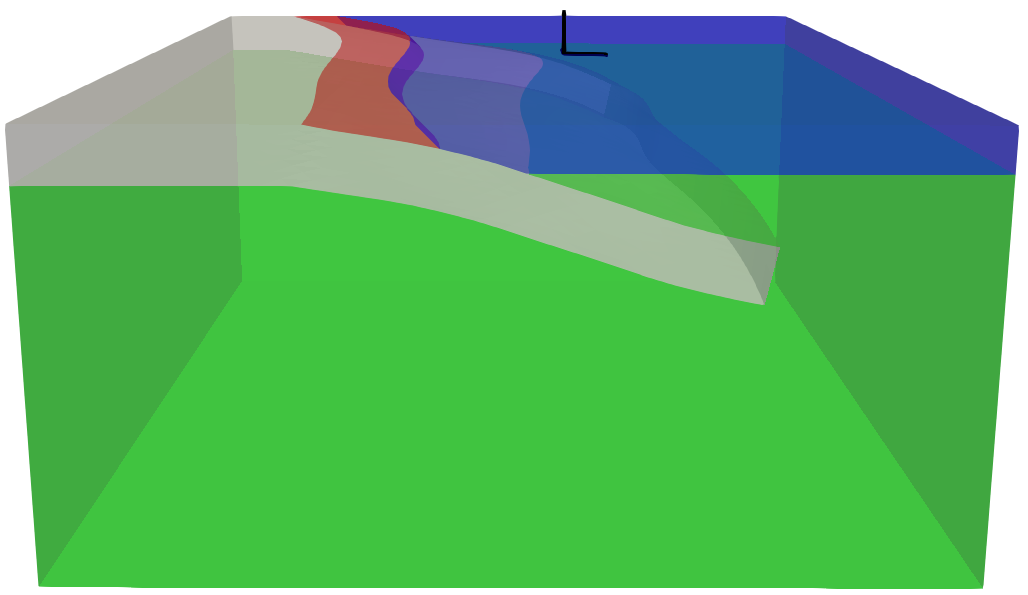
\includegraphics[width=4.5in]{examples/figs/subduction3d_geometry}};
    \begin{scope}[x={(image.south east)},y={(image.north west)}]
      \node[anchor=west, annotation] (xneg) at (-0.2,0.5) {+2.0 m};
      \draw[>=latex, ->, ultra thick, annotation] (xneg) -- (0.0,0.5);
      \node[anchor=east, annotation] (xpos) at (+1.2,0.5) {-2.0 m};
      \draw[>=latex, ->, ultra thick, annotation] (xpos) -- (1.0,0.5);
    \end{scope}
  \end{tikzpicture}
  \caption{Diagram of Step 1: Axial compression. This static
    simulation uses Dirichlet boundary conditions with axial
    compression in the east-west (x-direction), roller boundary
    conditions on the north, south, and bottom boundaries, and purely
    elastic properties.}
  \label{fig:example:subduction:3d:step01:diagram}
\end{figure}

The \filename{pylithapp.cfg} file creates an array of five boundary
conditions, which impose zero displacements by default. We overwrite
this behavior in the \filename{step01.cfg} file for the -x and +x
boundaries using spatial databases with a single uniform displacement
value to create the axial compression:
\begin{cfg}
# -x face
<h>[pylithapp.problem.bc.x_neg]</h>
<f>db_initial</f> = spatialdata.spatialdb.UniformDB
<p>db_initial.label</p> = Dirichlet BC on -x
<p>db_initial.values</p> = [displacement-x]
<p>db_initial.data</p> = [+2.0*m]

# +x face
<h>[pylithapp.problem.bc.x_pos]</h>
<f>db_initial</f> = spatialdata.spatialdb.UniformDB
<p>db_initial.label</p> = Dirichlet BC on +x
<p>db_initial.values</p> = [displacement-x]
<p>db_initial.data</p> = [-2.0*m]
\end{cfg}

As discussed in Section~\vref{sec:example:subduction:3d:organization},
we use \filename{mat\_elastic.cfg} to specify the parameters
associated with linear, isotropic elastic bulk constitutive models for
all of the materials for convenient reuse across several different
simulations.
\begin{cfg}
<h>[pylithapp.problem.materials]</h>
<f>slab</f> = pylith.materials.ElasticIsotropic3D
<f>wedge</f> = pylith.materials.ElasticIsotropic3D
<f>crust</f> = pylith.materials.ElasticIsotropic3D
<f>mantle</f> = pylith.materials.ElasticIsotropic3D

# Slab
<h>[pylithapp.problem.materials.slab]</h>
<f>db_properties</f> = spatialdata.spatialdb.SimpleDB
<p>db_properties.label</p> = Properties for subducting slab
<p>db_properties.iohandler</p>.filename = spatialdb/mat_slab_elastic.spatialdb

# Wedge
<h>[pylithapp.problem.materials.wedge]</h>
<f>db_properties</f> = spatialdata.spatialdb.SimpleDB
<p>db_properties.label</p> = Properties for accretionary wedge
<p>db_properties.iohandler.filename</p> = spatialdb/mat_wedge_elastic.spatialdb

# Mantle
<h>[pylithapp.problem.materials.mantle]</h>
<f>db_properties</f> = spatialdata.spatialdb.SimpleDB
<p>db_properties.label</p> = Properties for mantle
<p>db_properties.iohandler.filename</p> = spatialdb/mat_mantle_elastic.spatialdb

# Crust
<h>[pylithapp.problem.materials.crust]</h>
<f>db_properties</f> = spatialdata.spatialdb.SimpleDB
<p>db_properties.label</p> = Properties for continental crust
<p>db_properties.iohandler.filename</p> = spatialdb/mat_crust_elastic.spatialdb
\end{cfg}
We specify different elastic properties for each material
(slab, wedge, mantle, and crust) using \object{SimpleDB} spatial
databases with a single point to specify uniform properties within a
material. We choose \object{SimpleDB} rather than \object{UniformDB},
because we will reuse some of these spatial databases for the elastic
properties when we use linear Maxwell viscoelastic constitutive model.

The remaining parameters in the \filename{step01.cfg} file are mostly
associated with setting filenames for all of the various output,
including all of the parameters used and version information in a JSON
file, a file reporting the progress of the simulation and estimated
time of completion, and the filenames for the HDF5 files (the
corresponding Xdmf files will use the same filename with the
\filename{.xmf} suffix).

We run this example by typing
\begin{shell}
$$ pylith step01.cfg mat_elastic.cfg
\end{shell}
The problem will produce ten pairs of HDF5/Xdmf files. The HDF5
files contain the data and the Xdmf files contain the metadata required
by ParaView and Visit (and other visualization tools that
use Xdmf files) to access the mesh and data sets in the HDF5 files.
The files include the solution over the domain and ground surface
(two pairs of files), and physical properties, stress, and strain within
each material (eight pairs of files). 

Figure \vref{fig:example:subduction:3d:step01}, which was created
using the ParaView Python script \filename{plot\_dispvec.py}, displays
the magnitude of the displacement field arrows showing the direction
and magnitude of the deformation. Material properties with a positive
Poisson's ratio result in vertical deformation along with the axial
compression. The variations in material properties among the
properties result in local spatial variations that are most evident in
the horizontal displacement components.

\begin{figure}
  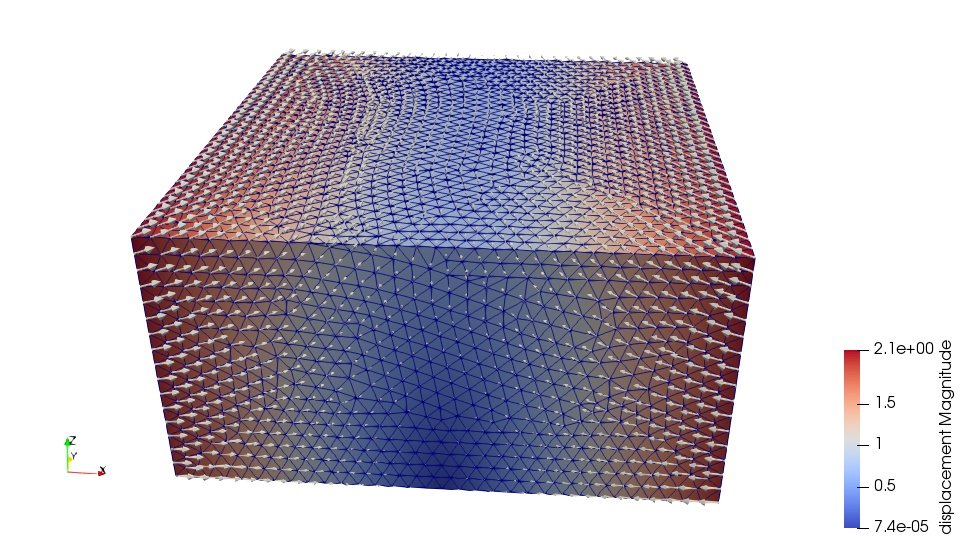
\includegraphics[width=5.0in]{examples/figs/subduction3d_step01_soln}
  \caption{Solution over the domain for Step 1. The colors indicate
    the magnitude of the displacement and the arrows indicate the
    direction with the length of each arrow equal to 10,000 times the
    magnitude of the displacement.}
  \label{fig:example:subduction:3d:step01}
\end{figure}


There are three different ways you can run this Python script to view
the solution:
\begin{enumerate}
\item From a shell (terminal window) start ParaView via the command line from the
  \filename{examples/3d/subduction} directory. Within the ParaView GUI, select
  \object{Tools}$\rightarrow$\object{Python Shell}, click on the
  \object{Run Script} button, and navigate to the \filename{viz}
  directory and select the \filename{plot\_dispvec.py} file.

\item From a shell (terminal window) start ParaView via the command line from the
  \filename{examples/3d/subduction} directory adding the
  \filename{-{}-script=viz/plot\_dispvec.py} command line argument.
\begin{shell}
# Make sure you are in the examples/3d/subduction directory.
$$ PATH_TO_PARAVIEW/paraview --script=viz/plot_dispvec.py
\end{shell}
\item Run the ParaView Python script directly from a shell (terminal
  window) via the command line. You can use command line arguments to
  set user-specified parameters.
\begin{shell}
# Make sure you are in the examples/3d/subduction directory.
# We show the optional command line arguments in square brackets.  
$$ ./viz/plot_dispvec.py [--vector-scale=10.0e+4] [--sim=step01.cfg} [--screenshot=FILE]
\end{shell}
\end{enumerate}

\tip{Running the ParaView Python script from within the ParaView GUI
  allows further manipulation of the data, which is not possible when
  running the ParaView Python script outside the ParaView
  GUI.}

\tip{In order to change the user-specified parameters in the ParaView
  Python scripts when running them from within the ParaView GUI, you
  must edit the file in an external text editor before running the
  script. If you are running these script from outside the ParaView
  GUI, you can simply use command line argument to change the
  user-specified parameters.}

\important{The ParaView Python scripts run Python via
  \filename{pvpython}, which is a customized version of the Python
  interpreter included in the ParaView distribution. This is different
  from Python provided with your operating system and the one included
  in the PyLith distribution.}

  
\subsubsection{Exercises}


\begin{itemize}
\item Run PyLith again and add
  \filename{solver\_algebraicmultigrid.cfg} as an argument on the
  command line to switch to the
  algebraic multigrid preconditioner.
  \begin{itemize}
  \item Using the PETSc log summary to compare the runtime and
    memory use between the original LU preconditiner and the ML
    algebraic multigrid preconditioner. Hint: The algebraic
    multigrid preconditioner is faster.
  \item Run the simulation again with the algebraic multigrid
    preconditioner using multiple cores via the
    \commandline{-{}-nodes=NCORES} argument, replacing
    \commandline{NCORES} with 2 or up to the number of cores on your
    machine. Examine the PETSc log summary for the various runs to
    see how the time spent at varies stages changes with the number
    of cores. Make a plot of runtime versus the number of
    cores.
  \end{itemize}
\item Adjust the material properties in the spatial databases so that the slab is stiffer and
  the wedge is more compliant. What happens to the solution if you make the
  materials nearly incompressible? Does this also affect the rate of
  convergence of the linear solve?
\item Change the Dirichlet boundary conditions to impose pure shear
  instead of axial compression. Hint: You will need to change the
  boundary conditions on the east, west, north, and south
  boundaries.
\end{itemize}
    

% ----------------------------------------------------------------------
\subsection{Step 2: Prescribed Coseismic Slip and Postseismic Relaxation}
\label{sec:example:subduction:3d:step02}

In this example we model the postseismic relaxation of the deep slab
and mantle resulting from coseismic slip on a fault patch in the
central portion of the subduction (top of the slab) interface. For
simplicity we will prescribed uniform slip on the fault patch and use
a linear Maxwell viscoelastic constitutive models for the slab and
mantle. As the lateral and bottom boundaries are far from the
earthquake source, we use roller boundary conditions on these
boundaries. We do not expect significant relaxation of stresses on the
shallow part of the slab, so we impose a depth-dependent
viscosity. Figure~\ref{fig:example:subduction:3d:step02:diagram}
summarizes the problem description.

\todo{brad}{Add annotation to figure.}
\begin{figure}[htbp]
  \begin{tikzpicture}
    \tikzstyle{annotation} = [black];
    \node[anchor=south west,inner sep=0] (image) at (0,0) {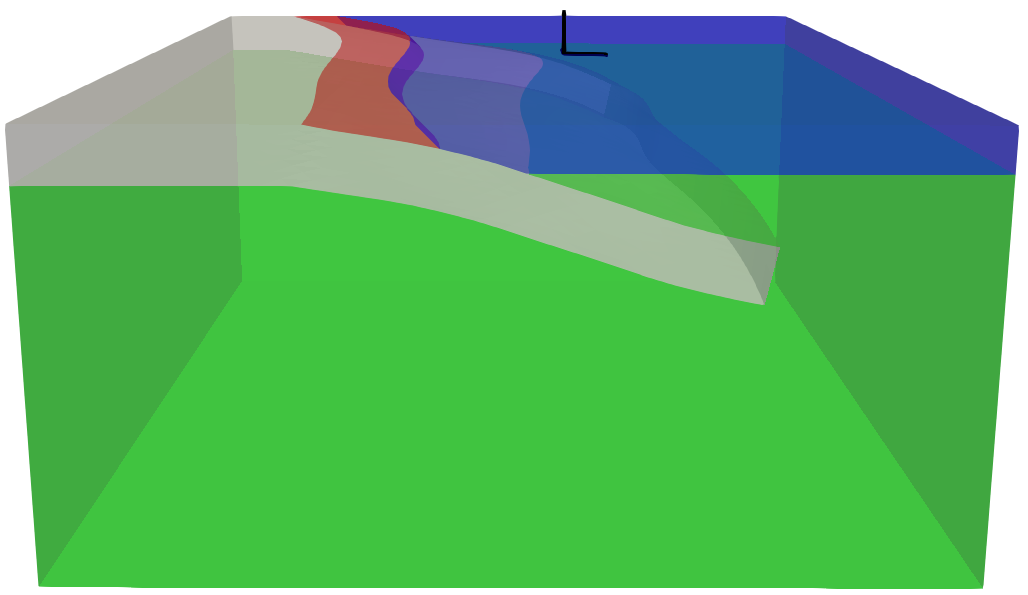
\includegraphics[width=4.5in]{examples/figs/subduction3d_geometry}};
    \begin{scope}[x={(image.south east)},y={(image.north west)}]
      \node at (0.5,0.5) {{\bf\LARGE ADD ANNOTATION}};
      %\node[anchor=west, annotation] (xneg) at (-0.2,0.5) {+2.0 m};
      %\draw[>=latex, ->, ultra thick, annotation] (xneg) -- (0.0,0.5);
      %\node[anchor=east, annotation] (xpos) at (+1.2,0.5) {-2.0 m};
      %\draw[>=latex, ->, ultra thick, annotation] (xpos) -- (1.0,0.5);
    \end{scope}
  \end{tikzpicture}
  \caption{Diagram of Step 2: Prescribed coseismic slip and
    postseismic relaxation. This quasistatic simulation prescribes
    uniform slip on the central rupture patch on the top of the slab,
    depth-dependent viscoelastic relaxation in the slab and mantle,
    and roller boundary conditions on the lateral (north, south, east,
    and west) and bottom boundaries.}
  \label{fig:example:subduction:3d:step02:diagram}
\end{figure}

The \filename{pylithapp.cfg} completely specifies the Dirichlet roller
boundary conditions on the five boundaries, so we do not include any
boundary condition information in \filename{step02.cfg}. As discussed
in Section~\vref{sec:example:subduction:3d:organization}, we bundle
the parameters for specification of an elastic crust and wedge and
viscoelastic slab and mantle in \filename{mat\_viscoelastic.cfg}.

% Materials
We describe the properties of the linear, isotropic Maxwell
viscoelastic constitutive model using viscosity in addition to the Vp,
Vs, and density used to describe purely linear, isotropic elastic
models. Rather than create a database with all four of these
parameters, we leverage the \object{SimpldDB} spatial databases used
by \filename{mat\_elastic.cfg} for the elastic properties and simply
create a single new spatial database with the depth-dependent
viscosity for the slab and mantle. We use the \object{CompositeDB}
spatial database to combine these two spatial databases into a single
spatial database with the material properties. Rather than using a
\object{SimpleDB} for the depth-dependent viscosity, we use a
\object{SimpleGridDB} spatial database
(\filename{spatialdb/mat\_viscosity}), which provides faster
interpolation using a bilinear search algorithm along each coordinate
direction. We use a very large viscosity at depths above 20 km to give
behavior that is essentially elastic and decrease it so the Maxwell
relaxation time (viscosity divided by the shear modulus) is
approximately 200 years at a depth of 30 km, 100 years at a depth of
100 km, and 50 years at a depth of 400 km. Using linear interpolation
results in a piecewise linear variation in the viscosity with depth.

\tip{The \object{SimpleGridDB} should be used whenever the points in a
  spatial database can be described with a logically rectangular
  grid. The grid points along each direction do not need to be
  uniformly spaced.}

In setting the parameters for the \object{CompositeDB} in
\filename{mat\_viscoelastic.cfg}, we specify which properties are
contained in each of the two spatial databases in the composite
database and the type and parameters for each of those spatial
databases. For the slab we have:
\begin{cfg}
<h>[pylithapp.problem.materials.slab]</h>
<f>db_properties</f> = spatialdata.spatialdb.CompositeDB
<p>db_properties.label</p> = Composite spatial database for slab material properties

<h>[pylithapp.timedependent.materials.slab.db_properties]</h>
# Elastic properties
<p>values_A</p> = [density, vs, vp]
<f>db_A</f> = spatialdata.spatialdb.SimpleDB
<p>db_A.label</p> = Elastic properties
<p>db_A.iohandler.filename</p> = spatialdb/mat_slab_elastic.spatialdb

# Viscoelastic properties
<p>values_B</p> = [viscosity]
<f>db_B</f> = spatialdata.spatialdb.SimpleGridDB
<p>db_B.label</p> = Linear Maxwell viscoelatic properties
<p>db_B.filename</p> = spatialdb/mat_viscosity.spatialdb
<p>db_B.query_type</p> = linear
\end{cfg}

In the simulation specific parameter file \filename{step02.cfg}, we
specify the parameters for the quasistatic time stepping, the
coesismic rupture, and the filenames for output. By default, PyLith
will use implicit time stepping with uniform time steps, so we need
only specify the duration and time step size.
\begin{cfg}
<h>[pylithapp.problem.formulation.time_step]</h>
# Define the total time for the simulation and the time step size.
<p>total_time</p> = 200.0*year
<p>dt</p> = 10.0*year
\end{cfg}

In prescribing coseismic slip on the single fault patch, we create an
array with one fault interface and then set its parameters. Because
the edges of the central fault patch are buried within the domain, we
need to specify the nodeset that corresponds to the buried edges as
well as the nodeset for the entire fault surface. This ensures that
PyLith inserts the cohesive cells and properly terminates the fault
surface at the edges. Just as we do for the boundary conditions and
materials, we create an array of components (in this case an array
with one fault interface, \facility{slab}, and then refer to those
components by name, \facility{pylithapp.problem.interfaces.slab}. We
must also set the discretization information for the fault.
\begin{cfg}
<h>[pylithapp.problem]</h>
# We prescribe slip on the slab fault patch.
<f>interfaces</f> = [slab]

<h>[pylithapp.problem.interfaces]</h>
<f>slab</f> = pylith.faults.FaultCohesiveKin ; Default

<h>[pylithapp.problem.interfaces.slab]</h>
<p>label</p> = fault_slabtop_patch ; Nodeset for entire fault surface
<p>edge</p> = fault_slabtop_patch_edge ; Nodeset for buried edges

# We must define the quadrature information for fault cells.
# The fault cells are 2D (surface).
<f>quadrature.cell</f> = pylith.feassemble.FIATSimplex
<p>quadrature.cell.dimension</p> = 2
\end{cfg}

Prescribing the coseismic slip distribution on the fault involves
specifying an origin time for the rupture (default is 0.0), and a slip
time function along with its
parameters. In this case, we treat the earthquake rupture as just the
coseismic slip happening in one time step, so we use a step function
for the slip time function (which is the default). The parameters
include the final slip and slip initiation time. Because we want
uniform slip and a uniform rise time, we use \object{UniformDB}
spatial databases for both of these. Note that we specify oblique slip
with 1.0 m of right-lateral motion and 4.0 m of reverse motion.
\begin{cfg}
<h>[pylithapp.problem.interfaces.slab.eq_srcs.rupture.slip_function]</h>
<f>slip</f> = spatialdata.spatialdb.UniformDB
<p>slip.label</p> = Final slip
<p>slip.values</p> = [left-lateral-slip, reverse-slip, fault-opening]
<p>slip.data</p> = [-1.0*m, 4.0*m, 0.0*m] 

<f>slip_time</f> = spatialdata.spatialdb.UniformDB
<p>slip_time.label</p>  = Slip initiation time
<p>slip_time.values</p> = [slip-time]
<p>slip_time.data</p> = [9.999*year] ; Use 10*year-small value to account for roundoff errors

<h>[pylithapp.problem.interfaces.slab.output]</h>
<f>writer</f> = pylith.meshio.DataWriterHDF5
<p>writer.filename</p> = output/step02-fault-slab.h5
<p>vertex_info_fields</p> = [normal_dir, strike_dir, dip_dir, final_slip_rupture, slip_time_rupture]
\end{cfg}

We run this example by typing
\begin{shell}
$$ pylith step02.cfg mat_viscoelastic.cfg solver_fieldsplit.cfg
\end{shell}

Figure \vref{fig:example:subduction:3d:step02}, which was created
using the ParaView Python script \filename{plot\_dispwarp.py},
displays the magnitude of the displacement field exaggerated by a
factor of 10,000 at the final time step (200 yr).  The shallow
fault results in deformation that is localized over a small region.

\begin{figure}
  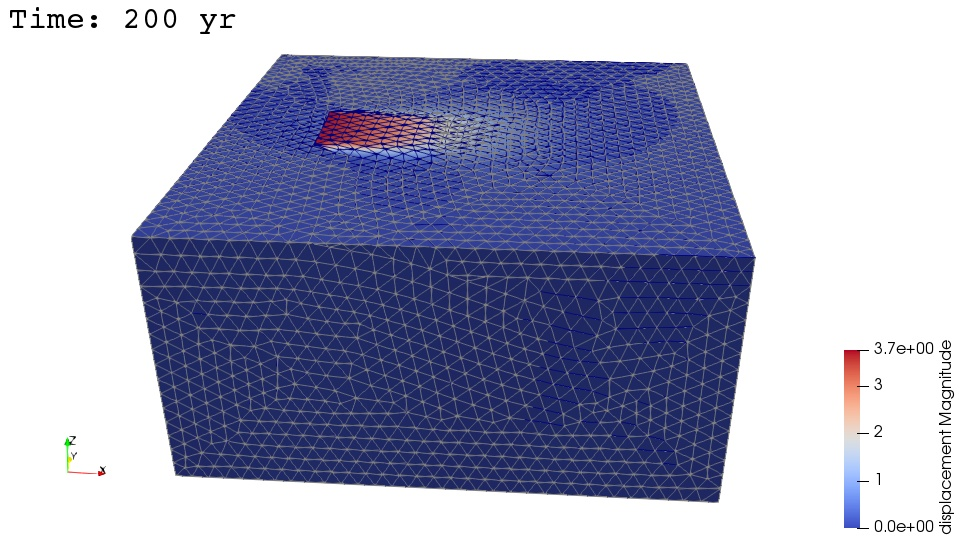
\includegraphics[width=5.0in]{examples/figs/subduction3d_step02_soln}
  \caption{Solution over the domain for Step 2 at $t = 200 \mathrm{yr}$. The
    colors indicate the magnitude of the displacement and we have
    exaggerated the deformation by a factor of 10,000.}
  \label{fig:example:subduction:3d:step02}
\end{figure}


\subsubsection{Exercises}

\begin{itemize}
\item Change the slip from the top of the slab to the splay fault
  rupture patch. Hint: Identify the nodesets for the splay fault
  patch.
\item Create simulataneous rupture on the central patch for the splay
  fault and top of the slab.
\item Prescribe coseismic slip on the central patch for splay fault
  and the top of the slab below the intersection with the splay fault.
  \begin{itemize}
  \item Implement this without changing the any of the nodesets. Hint:
    You will need to create two fault interfaces. What do you notice
    about the slip at the intersection between the splay fault and slab?
  \item Add nodesets in CUBIT/Trelis to create a uniform coseismic
    slip distribution across the splay fault and on the slab interface
    below the splay fault.
  \end{itemize}
\end{itemize}


% ----------------------------------------------------------------------
\subsection{Step 3: Prescribed Aseismic Creep and Interseismic Deformation}
\label{sec:example:subduction:3d:step03}

We now increase the complexity of our fault model by simulating the
interseismic deformation associated with the subducting slab. We
approximate the motion of the Juan de Fuca Plate subducting under the
North American Plate by introducing aseismic slip (creep) on the
bottom of the slab and the deeper portion of the top of the slab; we
keep the interface between the top of the slab and the accretionary
wedge and shallow crust locked. As in Step 2, we will use the linear
Maxwell viscoelastic constitutive model for the slab and mantle.
Figure~\ref{fig:example:subduction:3d:step03:diagram} summarizes the
problem description.

\todo{brad}{Add annotation to figure.}
\begin{figure}[htbp]
  \begin{tikzpicture}
    \tikzstyle{annotation} = [black];
    \node[anchor=south west,inner sep=0] (image) at (0,0) {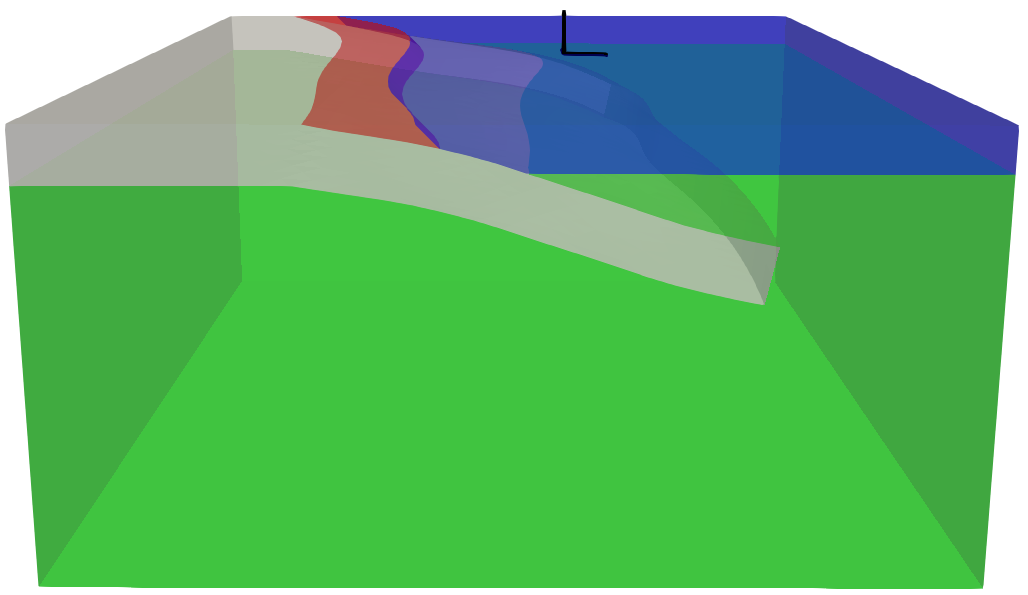
\includegraphics[width=4.5in]{examples/figs/subduction3d_geometry}};
    \begin{scope}[x={(image.south east)},y={(image.north west)}]
      \node at (0.5,0.5) {{\bf\LARGE ADD ANNOTATION}};
      %\node[anchor=west, annotation] (xneg) at (-0.2,0.5) {+2.0 m};
      %\draw[>=latex, ->, ultra thick, annotation] (xneg) -- (0.0,0.5);
      %\node[anchor=east, annotation] (xpos) at (+1.2,0.5) {-2.0 m};
      %\draw[>=latex, ->, ultra thick, annotation] (xpos) -- (1.0,0.5);
    \end{scope}
  \end{tikzpicture}
  \caption{Diagram of Step 3: Prescribed aseismic slip (creep) and
    interseismic deformation for the subducting slab. We precsribed
    steady, uniform creep on the
    bottom of the slab and deeper portion of the top of the slab. We
    impose roller Dirichlet boundary conditions on the lateral and
    bottom boundaries, except where they overlap with the fault
    interfaces for the slab.}
  \label{fig:example:subduction:3d:step03:diagram}
\end{figure}

% Fault
With slip on the top and bottom of the slab, our fault interfaces
array contains two components, one for the top of the slab,
\facility{slab\_top}, and one for the bottom of the slab,
\facility{slab\_bottom}. We use the \object{FaultCohesiveKin}
object for each of these interfaces since we want to prescribe the
slip.
\begin{cfg}
<h>[pylithapp.problem]</h>
<f>interfaces</f> = [slab_top, slab_bottom]

<h>[pylithapp.problem.interfaces]</h>
<f>slab_top</f> = pylith.faults.FaultCohesiveKin
<f>slab_bottom</f> = pylith.faults.FaultCohesiveKin
\end{cfg}

% Bottom of slab
We specify the \property{id} used to identify the cohesive cells for
this fault so that it is unique among all materials and faults. We
also specify the appropriate nodesets identifying the entire fault
surface and the buried edges.  Some portions of the bottom of the slab
are perfectly horizontal, so our procedure that uses the vertical
direction and the fault normal to set the along-strike and up-dip
shear components breaks down. We remedy this by tweaking the
\property{up\_dir} direction from being completely vertical (0,0,1) to
tilting slightly to the west. This results in consistent along-strike
and up-dip directions across the fault surface. For the aseismic slip
we use a constant slip rate time function (\object{ConstRateSlipFn})
with \object[UniformDB} spatial databases to specify the constant,
uniform oblique slip rate of 2.0 cm/yr of left-lateral motion and 4.0
cm/yr of normal motion. Note that slip on the bottom of the subducting
slab has the opposite sense of motion as that on the top of the slab.
\begin{cfg}
<h>[pylithapp.problem.interfaces.slab_bottom]</h>
<p>id</p> = 100 ; Must be different from ids used for materials
<p>label</p> = fault_slabbot ; Nodeset for the entire fault surface
<p>edge</p> = fault_slabbot_edge ; Nodeset for the buried edges
# Give slight westward tilt to the up_dir to avoid ambigious
# directions for the shear components on the horizontal portions of the
# fault.
<p>up_dir</p> = [-0.1,0,0.9]

# We must define the quadrature information for fault cells.
# The fault cells are 2D (surface).
<f>quadrature.cell</f> = pylith.feassemble.FIATSimplex
<p>quadrature.cell.dimension</p> = 2

# Use the constant slip rate time function.
<f>eq_srcs.rupture.slip_function</f> = pylith.faults.ConstRateSlipFn

# The slip time and final slip are defined in spatial databases.
<h>[pylithapp.problem.interfaces.slab_bottom.eq_srcs.rupture.slip_function]</h>
<f>slip_rate</f> = spatialdata.spatialdb.UniformDB
<p>slip_rate.label</p> = Slab bottom slip rate.
<p>slip_rate.values</p> = [left-lateral-slip, reverse-slip, fault-opening]
<p>slip_rate.data</p> = [+2.0*cm/year, -4.0*cm/year, 0.0*cm/year]

<f>slip_time</f> = spatialdata.spatialdb.UniformDB
<p>slip_time.label</p>  = Slip initiation time
<p>slip_time.values</p> = [slip-time]
<p>slip_time.data</p> = [0.0*year] 

<h>[pylithapp.problem.interfaces.slab_bottom.output]</h>
<f>writer</f> = pylith.meshio.DataWriterHDF5
<p>writer.filename</p> = output/step03-fault-slabbot.h5
<p>vertex_info_fields</p> = [normal_dir, strike_dir, dip_dir]
\end{cfg}

% Top of slab
The parameters for the top of the slab closely resemble those for the
bottom of the slab. The main difference is that we use a
\object{SimpleGridDB} to define a depth variation in the slip
rate. The fault is locked at depths above 45 km and increases linearly
to the same slip rate as the bottom of the slab at a depth of 60 km.
\begin{cfg}
<h>[pylithapp.problem.interfaces.slab_top]</h>
<p>id</p> = 101 ; Must be different from ids used for materials
<p>label</p> = fault_slabtop ; Nodeset for the entire fault surface
<p>edge</p> = fault_slabtop_edge ; Nodeset for the buried edges

# We must define the quadrature information for fault cells.
# The fault cells are 2D (surface).
<f>quadrature.cell</f> = pylith.feassemble.FIATSimplex
<p>quadrature.cell.dimension</p> = 2

# Use the constant slip rate time function.
<f>eq_srcs.rupture.slip_function</f> = pylith.faults.ConstRateSlipFn

# The slip time and final slip are defined in spatial databases.
<h>[pylithapp.problem.interfaces.slab_top.eq_srcs.rupture.slip_function]</h>
<f>slip_rate</f> = spatialdata.spatialdb.SimpleGridDB
<p>slip_rate.label</p> = Slab top slip rate.
<p>slip_rate.filename</p> = spatialdb/fault_slabtop_creep.spatialdb
<p>slip_rate.query_type</p> = linear

<f>slip_time</f> = spatialdata.spatialdb.UniformDB
<p>slip_time.label</p>  = Slip initiation time
<p>slip_time.values</p> = [slip-time]
<p>slip_time.data</p> = [0.0*year]

<h>[pylithapp.problem.interfaces.slab_top.output]</h>
<f>writer</f> = pylith.meshio.DataWriterHDF5
<p>writer.filename</p> = output/step03-fault-slabtop.h5
<p>vertex_info_fields</p> = [normal_dir, strike_dir, dip_dir]
\end{cfg}

% Boundary conditions
PyLith does not support an overlap between Dirichlet boundary
conditions and fault interfaces, so we use nodesets that exclude
vertices on the faults for the -x, -y, and +y boundaries rather than
the nodesets that include all vertices on those boundaries.
\begin{cfg}
# -x face
<h>[pylithapp.problem.bc.x_neg]</h>
<p>label</p> = boundary_xneg_nofault

# -y face
<h>[pylithapp.problem.bc.y_neg]</h>
<p>label</p> = boundary_yneg_nofault

# +y face
<h>[pylithapp.problem.bc.y_pos]</h>
<p>label</p> = boundary_ypos_nofault
\end{cfg}

We run this example by typing
\begin{shell}
$$ pylith step03.cfg mat_viscoelastic.cfg solver_fieldsplit.cfg
\end{shell}

Figure \vref{fig:example:subduction:3d:step03}, which was created
using the ParaView Python script \filename{plot\_dispwarp.py}, shows
the deformation exaggerated by a factor of 5,000 at the final time
step of t=200*yr. Notice that there are some local edge effects
associated with the unconstrained degrees of freedom at the
intersection of the boundaries and fault surfaces.

\begin{figure}
  %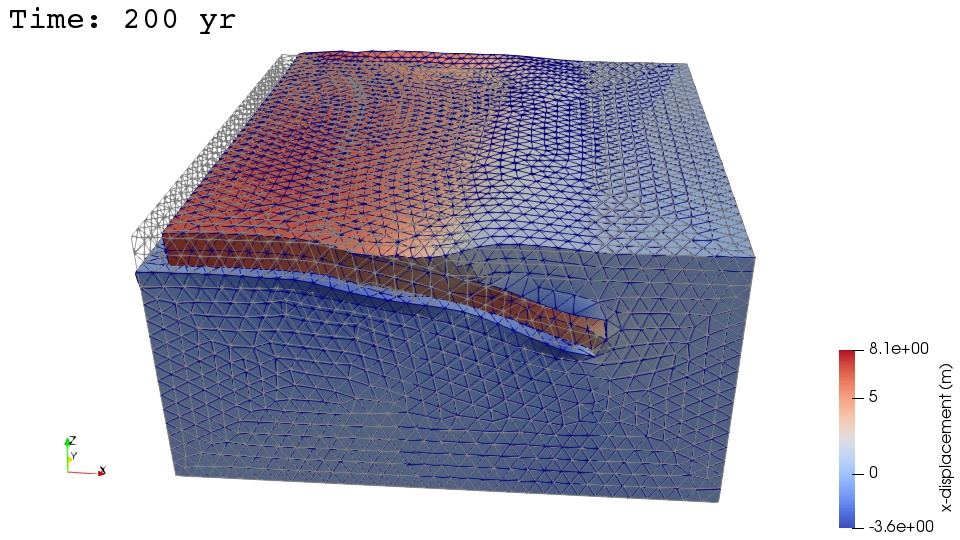
\includegraphics[width=5.0in]{examples/figs/subduction3d_step03_soln}
  \caption{Solution over the domain for Step 2 at $t=200 \mathrm{yr}$. The colors indicate
    the x-displacement and we have exaggerated the
    deformation by a factor of 5,000.}
  \label{fig:example:subduction:3d:step03}
\end{figure}


\subsubsection{Exercises}

\begin{itemize}
\item Adjust the locking depth for the top of the slab. How does this
  affect the spatial distribution of the change in tractions on
  the fault interfaces?
\item Increase the rigidity of the slab and decrease the rigidity of
  the wedge and/or crust. How do these affect the change in tractions
  on the fault interfaces?
\end{itemize}


% ----------------------------------------------------------------------
\subsection{Step 4: Prescribed Earthquake Cycle}

\subsubsection{Exercises}

% Make lower slab + splay fault the primary fault surface and the
% upper slab (trench side of the splay fault) the secondary fault
% surface. Hint: You will need to create a nodesets in CUBIT that
% correspond to the primary and secondary fault surfaces.



% ----------------------------------------------------------------------
\subsection{Step 5: Spontaneous Rupture Driven by Subducting Slab}

\subsubsection{Exercises}

% ----------------------------------------------------------------------
\subsection{Step 6: Prescribed Slow-Slip Event}

This example simulates a simple slow slip event (SSE) on the
subduction interface that remains fixed spatially but increases its
amplitude with time. We assume a constant rake angle of 110 degrees,
and a time duration of 30 days. This problem requres the use of both a
spatial database to provide the spatial distribution of slip, and a
temporal database to describe the time evolution of slip. To create
these databases we provide the \filename{generate\_slowslip.py}
script, which is in the \filename{spatialdb} directory. Once you are
in the \filename{spatialdb} directory, run the script as follows:
\begin{shell}
$$ ./generate_slowslip.py
\end{shell}
This script reads parameters from \filename{generate\_slowslip.cfg} to
generate a Gaussian slip distribution in geographic coordinates, along
with a temporal database providing the slip amplitudes at different
times. The files created are:
\begin{itemize}
\item \filename{fault\_slabtop\_slowslip.spatialdb}: Spatial database
\item \filename{fault\_slabtop\_slowslip.timedb}: Temporal database
\end{itemize}

Note that \filename{fault\_slabtop\_slowslip.spatialdb} is a
\facility{SimpleGridDB}. This type of spatial database is very
efficient in cases where property values lie on a regular grid in 2 or
3 dimensions, since searches and interpolations reduce to a set of 1D
operations. Once the database files have been generated, it is
possible to run the example. There are a number of parameters that are
changed from or added to those in \filename{pylithapp.cfg}. We first
change the total simulation time to 30 days with a time step size of 2
days:
\begin{cfg}
<h>[pylithapp.problem.formulation.time_step]</h>
# Define the total time for the simulation and the time step size.
<p>total_time</p> = 30.0*day
<p>dt</p> = 2.0*day
\end{cfg}

The results in this example will be used to simulate output at cGPS
stations for example step07, so we modify the output manager to
provide output at synthetic cGPS stations as well as the entire domain
and ground surface:
\begin{cfg}
# For this problem, we want output over the entire domain, for the
# ground surface, and at simulated cGPS locations.
<h>[pylithapp.problem.implicit]</h>
<f>output</f> = [domain, subdomain, cgps_sites]

# Default output is for the entire domain.
# We need to set the type of output for the subdomain and points.
<f>output.subdomain</f> = pylith.meshio.OutputSolnSubset
<f>output.cgps_sites</f> = pylith.meshio.OutputSolnPoints
\end{cfg}

There are a number of parameters to change/modify related to the
fault. In particular, we change the default slip function to
\facility{pylith.faults.TimeHistorySlipFn}, which allows us to change
the slip amplitude as a function of time. We also use a
\facility{SimpleGridDB} to specify fault slip and linear interpolation
for the fault slip:
\begin{cfg}
<h>[pylithapp.problem]</h>
# We prescribe slip on the slab fault patch.
<f>interfaces</f> = [slab]

<h>[pylithapp.problem.interfaces]</h>
<f>slab</f> = pylith.faults.FaultCohesiveKin

<h>[pylithapp.problem.interfaces.slab]</h>
# Nodeset corresponding to the fault patch and buried edge.
<p>label</p> = fault_slabtop_patch
<p>edge</p> = fault_slabtop_patch_edge

# We must define the quadrature information for fault cells.
# The fault cells are 2D (surface).
<f>quadrature.cell</f> = pylith.feassemble.FIATSimplex
<p>quadrature.cell.dimension</p> = 2

# We use a time history slip function.
<h>[pylithapp.problem.interfaces.slab.eq_srcs.rupture]</h>
<f>slip_function</f> = pylith.faults.TimeHistorySlipFn

# The slip is defined in a spatial database.
<h>[pylithapp.problem.interfaces.slab.eq_srcs.rupture.slip_function]</h>
<f>slip</f> = spatialdata.spatialdb.SimpleGridDB
<p>slip.label</p> = Gaussian slip distribution for SSE
<p>slip.filename</p> = spatialdb/fault_slabtop_slowslip.spatialdb

# Use linear interpolation.
<p>slip.query_type</p> = linear

# We use a UniformDB to specify the slip initiation time.
<f>slip_time</f> = spatialdata.spatialdb.UniformDB
<p>slip_time.label</p> = Slip initiation time
<p>slip_time.values</p> = [slip-time]
<p>slip_time.data</p> = [0.0*year] 

# We use a temporal database to provide the slip time history.
<p>time_history.label</p> = Time history of slip
<p>time_history.filename</p> = spatialdb/fault_slabtop_slowslip.timedb
\end{cfg}

The final set of parameters involve output. The domain and subdomain
output are similar to previous examples:
\begin{cfg}
<h>[pylithapp.problem.formulation.output.domain]</h>
<f>writer</f> = pylith.meshio.DataWriterHDF5
<p>writer.filename</p> = output/step06-domain.h5

<h>[pylithapp.problem.formulation.output.subdomain]</h>
# Name of nodeset for top surface.
<p>label</p> = boundary_zpos
<f>writer</f> = pylith.meshio.DataWriterHDF5
<p>writer.filename</p> = output/step06-groundsurf.h5
\end{cfg}
For points output, we need to provide coordinate system information as
well as the name of the text file containing station names and
coordinates:
\begin{cfg}
# Specify output type, coordinate system, and station file for cgps_sites.
<h>[pylithapp.problem.formulation.output.cgps_sites]</h>
# We will use a geographic coordinate system for the cGPS sites file.
<f>coordsys</f> = spatialdata.geocoords.CSGeo
<p>coordsys.space_dim</p> = 3
<p>coordsys.datum_horiz</p> = WGS84
<p>coordsys.datum_vert</p> = mean sea level

# Use HDF5 output.
<f>writer</f> = pylith.meshio.DataWriterHDF5
<p>writer.filename</p> = output/step06-cgps_sites.h5

# Simulated cGPS station file.
<p>reader.filename</p> = cgps_sites.txt
\end{cfg}
The remainder of the settings are for fault and material output,
similar to other examples:
\begin{cfg}
# Fault output ------------------------------------------------------
<h>[pylithapp.problem.interfaces.slab.output]</h>
# Output fault results to HDF5 file.
writer = pylith.meshio.DataWriterHDF5
writer.filename = output/step06-fault-slab.h5

# We want both orientation and slip information in the information file.
vertex_info_fields = [normal_dir, strike_dir, dip_dir, final_slip_rupture]

# Material output ------------------------------------------------------
<h>[pylithapp.problem.materials.slab.output]</h>
<p>writer.filename</p> = output/step06-slab.h5

<h>[pylithapp.problem.materials.wedge.output]</h>
<p>writer.filename</p> = output/step06-wedge.h5

<h>[pylithapp.problem.materials.crust.output]</h>
<p>writer.filename</p> = output/step06-crust.h5

<h>[pylithapp.problem.materials.mantle.output]</h>
<p>writer.filename</p> = output/step06-mantle.h5
\end{cfg}

We use elastic properties for all materials, and custom solver
settings appropriate for a problem with a fault. We run the example by typing
\begin{shell}
$$ pylith step06.cfg mat_elastic.cfg solver_fieldsplit.cfg
\end{shell}
The problem will produce 13 pairs of HDF5/Xdmf files. In the data
files (those without a \filename{\_info} before the file suffix) there
are field values representing 15 time steps. The additional HDF5 file
that was not present in previous examples is
\filename{step06-cgps\_sites.h5}, which contains the displacements at
the simulated cGPS sites.

Figure \vref{fig:example:subduction:3d:step06}, which was created
using ParaView, shows the surface vertical displacement along with
horizontal displacement vectors at the cGPS sites, superimposed on
contours of the applied slip at t = 24 days.

\begin{figure}
  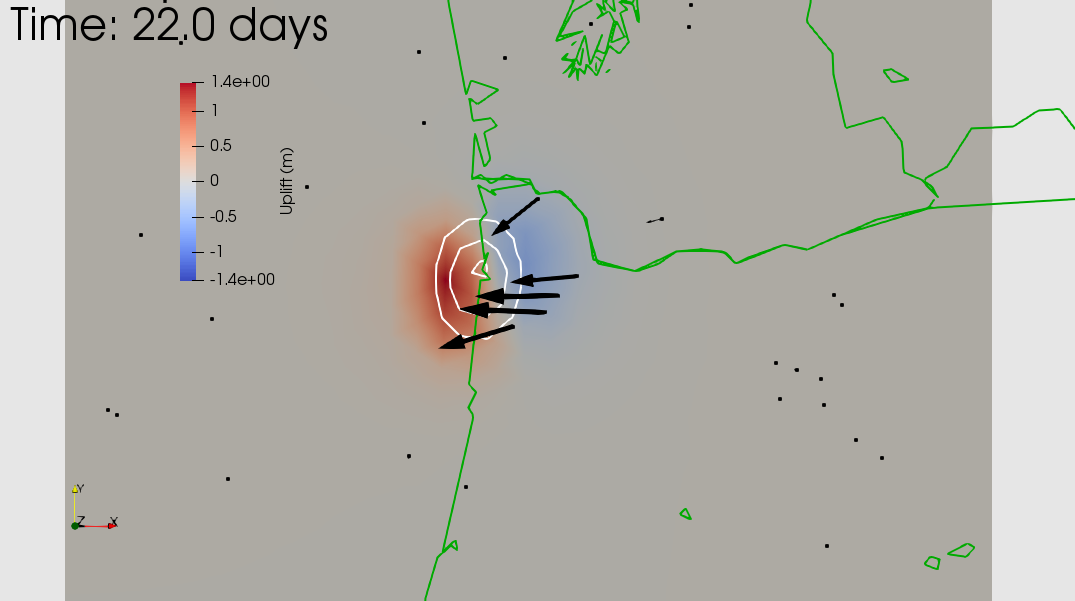
\includegraphics[width=4.5in]{examples/figs/subduction3d_step06_soln}
  \caption{Solution for Step 6. The colors indicate the vertical
    displacement, the vectors represent the horizontal displacements
    at simulated cGPS sites, and the contours represent the applied
    slip at t = 24 days.}
  \label{fig:example:subduction:3d:step06}
\end{figure}


\subsubsection{Exercises}

\begin{itemize}
\item Change spatial distribution and time history of slip.
  \begin{itemize}
  \item Edit \filename{generate\_slowslip.cfg} to change spatial and
    temporal distributions, and edit \filename{step06.cfg} to change the
    time duration and/or time step size.
  \end{itemize}
\item Add propagation of the slow slip (spatial variation of slip
  initiation time).
  \begin{itemize}
  \item Either alter Python script to produce a spatial database of
    slip initiation times, or write a new script. Can you produce a
    more realistic-looking slow slip event?
  \end{itemize}
\end{itemize}

% ----------------------------------------------------------------------
\subsection{Step 7: Inversion of Slow-Slip Event using 3-D Green's Functions}

This example is essentially a three-dimensional analog of
\vref{sec:example:greensfns2d}, and is a more realistic example of how
PyLith can be used to perform geodetic inversions. We use the output
of example step06 to create synthetic data. Once we have done this we
generate Green's functions to represent the geodetic responses at a
set of synthetic cGPS stations. Finally, we use the synthetic data and
Green's functions to perform an inversion, using the same generalized
inverse approach described in \vref{sec:example:greensfns2d:inversion}.

We first generate the synthetic data by using the script
\filename{make\_synthetic\_gpsdisp.py} in the top-level
directory. This script reads the parameters in
\filename{make\_synthetic\_gpsdisp.cfg} to generate synthetic data
from the selected time step with a specified amount of noise. The
point data output from example step06 is read, the specified time step
is selected, and the specified amount of noise is added to the
results. Run this script as:
\begin{shell}
$$ ./make_synthetic_gpsdisp.py
\end{shell}
This will create the following files:
\begin{description}
\item[\filename{cgps\_synthetic\_displacement.txt}] read by the
  inversion script.
\item[\filename{cgps\_synthetic\_displacement.vtk}] for visualization.
\end{description}

After we create the synthetic data, we generate the Green's
functions. We divide the Green's function generation into two sub-problems:
\begin{itemize}
 \item step07a:  Generate Green's functions corresponding to
   left-lateral slip on the subduction interface (slab top).
 \item step07b:  Generate Green's functions corresponding to
   updip slip on the subduction interface (slab top).
\end{itemize}
Note that the Green's functions could all be generated at the same
time; however, for real problems it is generally preferable to
separate the problems to improve runtimes (e.g., both problems can be
run simultaneously).

To generate the Green's functions we change the problem type from the
default \facility{timedependent} to \facility{greensfns}. We do this
on the command line. When we change the problem type to
\facility{greensfns}, PyLith automatically reads the file
\filename{greensfns.cfg}. This file contains non-default settings that
are common to both sub-problems. Note that since the problem type has
been changed from the default \facility{timedependent} to
\facility{greensfns}, the facility labels are changed. Also, since
\facility{problem} is a facility of \facility{pylithapp}, we no longer
need the \facility{pylithapp} prefix in this file. We first specify
the fault information:
\begin{cfg}
# Define the interfaces (slab) and provide a fault_id.
<h>[greensfns]</h>
<f>interfaces</f> = [slab]
<p>fault_id</p> = 100

# Switch fault to FaultCohesiveImpulses for generation of Green's functions.
<h>[greensfns.interfaces]</h>
<f>slab</f> = pylith.faults.FaultCohesiveImpulses

# Nodesets corresponding to the fault and its buried edge.
<h>[greensfns.interfaces.slab]</h>
<p>label</p> = fault_slabtop_patch
<p>edge</p> = fault_slabtop_patch_edge

# We must define the quadrature information for fault cells.
# The fault cells are 2D (surface).
<f>quadrature.cell</f> = pylith.feassemble.FIATSimplex
<p>quadrature.cell.dimension</p> = 2

# Spatial database for slip impulse amplitude.
<f>db_impulse_amplitude</f> = spatialdata.spatialdb.UniformDB
<p>db_impulse_amplitude.label</p> = Amplitude of fault slip impulses
<p>db_impulse_amplitude.values</p> = [slip]
<p>db_impulse_amplitude.data</p> = [1.0]
\end{cfg}

In addition to defining the fault information, we also set some output
information common to both sub-problems, writing addition info fields
for fault output, and turning off material output. If we left material
output turned on, we would end up with extremely large state variable
output files:
\begin{cfg}
<h>[greensfns.interfaces.slab.output]</h>
# Add impulse amplitude to fault info output.
<p>vertex_info_fields</p> = [normal_dir, strike_dir, dip_dir, impulse_amplitude]
<f>writer</f> = pylith.meshio.DataWriterHDF5

# Turn off output of state variables for materials.
<h>[greensfns.materials.slab.output]</h>
<p>cell_data_fields</p> = []

<h>[greensfns.materials.wedge.output]</h>
<p>cell_data_fields</p> = []

<h>[greensfns.materials.crust.output]</h>
<p>cell_data_fields</p> = []

<h>[greensfns.materials.mantle.output]</h>
<p>cell_data_fields</p> = []
\end{cfg}

The \filename{step07a.cfg} and \filename{step07b.cfg} files are
identical, except for the impulse type specification and file
names. Here are the fault parameters in \filename{step07a.cfg}:
\begin{cfg}
<h>[pylithapp.problem.interfaces.slab]</h>
# Impulses for left-lateral slip.
# Note that it is possible to apply both left-lateral and updip slip
# (impulse_dof = [0,1]), but we separate the impulses into two problems.
<p>impulse_dof</p> = [0]
\end{cfg}

In the output settings, we turn off output for the domain and ground
surface, provide coordinate system info for the simulated cGPS output,
and provide filenames:
\begin{cfg}
# Add cggs_sites to solution output.
<h>[pylithapp.problem.formulation]</h>
<f>output</f> = [domain, subdomain, cgps_sites]
<f>output.cgps_sites</f> = pylith.meshio.OutputSolnPoints

# Domain, subdomain, and cgs_sites
<h>[pylithapp.problem.formulation.output.domain]</h>
<p>writer.filename</p> = output/step07a-domain.h5
# Turn off data fields.
<p>vertex_data_fields</p> = []

<h>[pylithapp.problem.formulation.output.subdomain]</h>
<p>writer.filename</p> = output/step07a-groundsurf.h5
# Turn off data fields.
<p>vertex_data_fields</p> = []

<h>[pylithapp.problem.formulation.output.cgps_sites]</h>
<f>writer</f> = pylith.meshio.DataWriterHDF5
<p>writer.filename</p> = output/step07a-cgps_sites.h5

# Set coordinate system associated with file with cGPS sites
<p>reader.filename</p> = cgps_sites.txt
<f>coordsys</f> = spatialdata.geocoords.CSGeo
<p>coordsys.space_dim</p> = 3
<p>coordsys.datum_horiz</p> = WGS84
<p>coordsys.datum_vert</p> = mean sea level

# Fault
<h>[pylithapp.problem.interfaces.slab.output]</h>
<p>writer.filename</p> = output/step07a-fault-slab.h5

# Materials
<h>[pylithapp.problem.materials.slab.output]</h>
<p>writer.filename</p> = output/step07a-slab.h5

<h>[pylithapp.problem.materials.wedge.output]</h>
<p>writer.filename</p> = output/step07a-wedge.h5

<h>[pylithapp.problem.materials.crust.output]</h>
<p>writer.filename</p> = output/step07a-crust.h5

<h>[pylithapp.problem.materials.mantle.output]</h>
<p>writer.filename</p> = output/step07a-mantle.h5
\end{cfg}

You can run the two sub-problems as follows:
\begin{shell}
$$ pylith --problem=pylith.problems.GreensFns step07a.cfg
mat_elastic.cfg solver_fieldsplit.cfg
$$ pylith --problem=pylith.problems.GreensFns step07b.cfg
mat_elastic.cfg solver_fieldsplit.cfg
\end{shell}
\tip{To save runtime, run the two sub-problems simultaneously in
separate terminal windows. For a problem this size, this should work
fine on a laptop. For larger problems, this approach can still be
useful. Each sub-problem could be run simultaneously on several nodes
of a cluster, for example.}

After generating the synthetic data and Green's functions, we then
perform a simple inversion using the \filename{slip\_invert.py} script,
with parameters defined in \filename{slip\_invert.cfg}. This script
performs a set of linear inversions, in a manner similar to the
inversion in \vref{sec:example:greensfns2d:inversion}. This script is
in the top-level \filename{subduction} directory. From there, run the
script as follows:
\begin{shell}
$$ ./slip_invert.py
\end{shell}
This will create a number of files in the output directory. Note that
the HDF5 files have an associated \filename{.xmf} file to use with
ParaView:
\begin{description}
\item[\filename{step07-inversion-slip.h5}] This file may
  be used to visualize the predicted slip distributions for different
  values of the penalty weight.
\item[\filename{step07-inversion-displacement.h5}] This file may be used to
  visualize the predicted cGPS displacements for each solution.
\item[\filename{step07-inversion-summary.txt}] This file provides a summary
  of the inversion results for each value of the penalty weight.
\end{description}

When performing an inversion such as this, one approach is to find the
corner of the 'L-curve' when plotting the log of the weighted data
residual vs. the log of the penalty residual. This is viewed as the
point of diminishing returns for reducing the penalty
weight. Further reductions provide little improvement to the
weighted data residual, while providing a solution with less
regularization. A Python script has been provided in the
\filename{viz} subdirectory to plot this curve, assuming that the user
has the numpy and matplotlib Python packages installed. From the
\filename{viz} subdirectory, run this script as:
\begin{shell}
./plot_inversion_misfit.py
--summary=../output/step07-inversion-summary.txt
\end{shell}
This will produce a curve similar to that shown in Figure
\vref{fig:example:subduction:3d:step07:curve}
\begin{figure}
  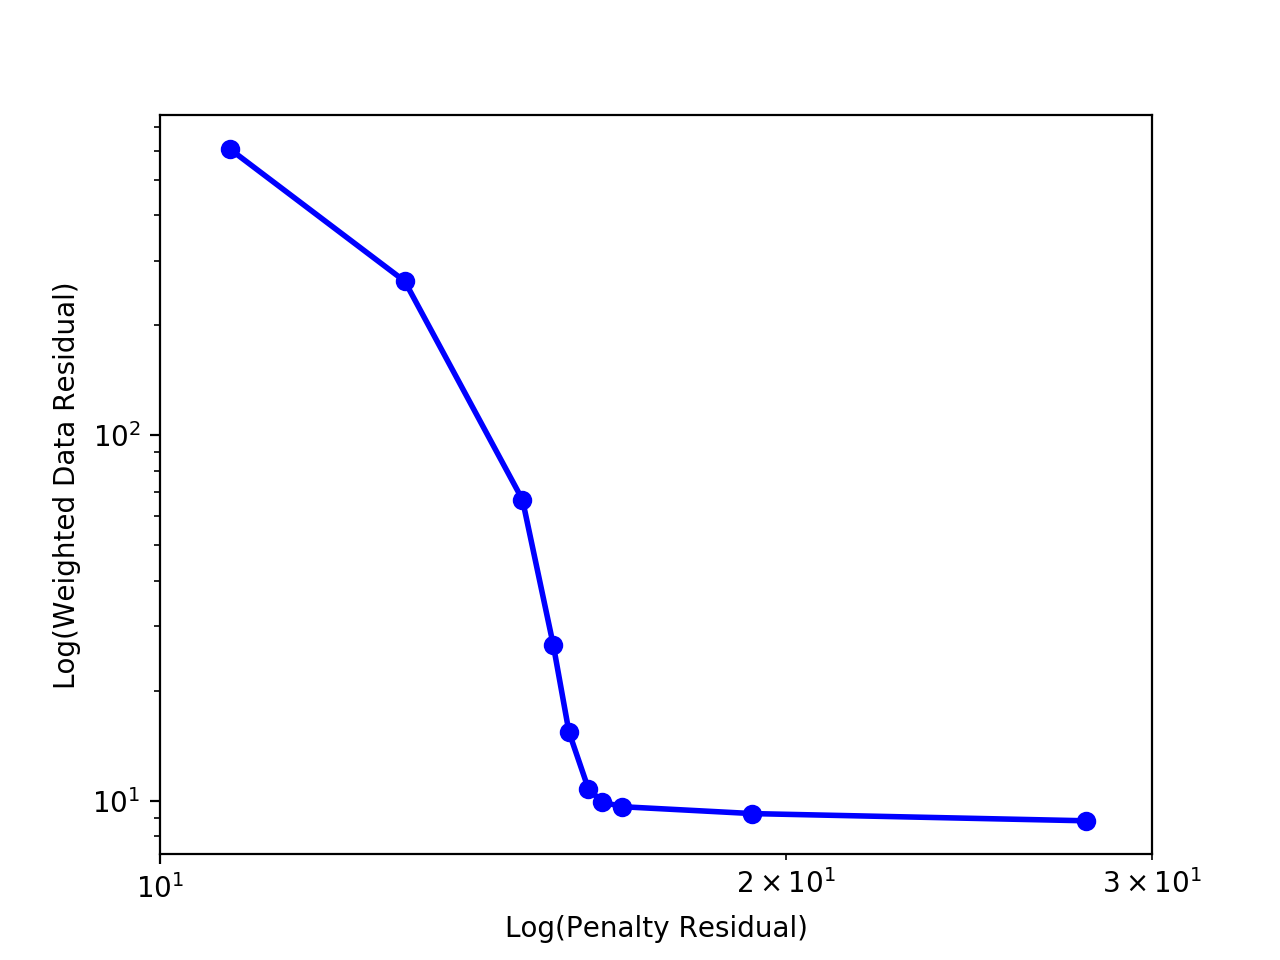
\includegraphics[width=4.5in]{examples/figs/subduction3d_step07_inverse_curve}
  \caption{Plot of the 'L-curve' for inversion in example step07. The
    'corner' of the L-curve would be about the third or fourth point
    from the right of the plot, representing a penalty weight of 0.5
    or 1.0 in our example. }
  \label{fig:example:subduction:3d:step07:curve}
\end{figure}

Once we have determined the optimal solution by analyzing the L-curve,
we can then visualize the results using ParaView. Figure
\vref{fig:example:subduction:3d:step07:invresults} shows the predicted
slip, the observed and predicted displacement vectors, and the slip
applied from example step06 for a penalty weight of 1.0. The data fit
is very good, and the predicted slip distribution is very close to the
applied slip, although the magnitude is slightly underestimated.
\begin{figure}
  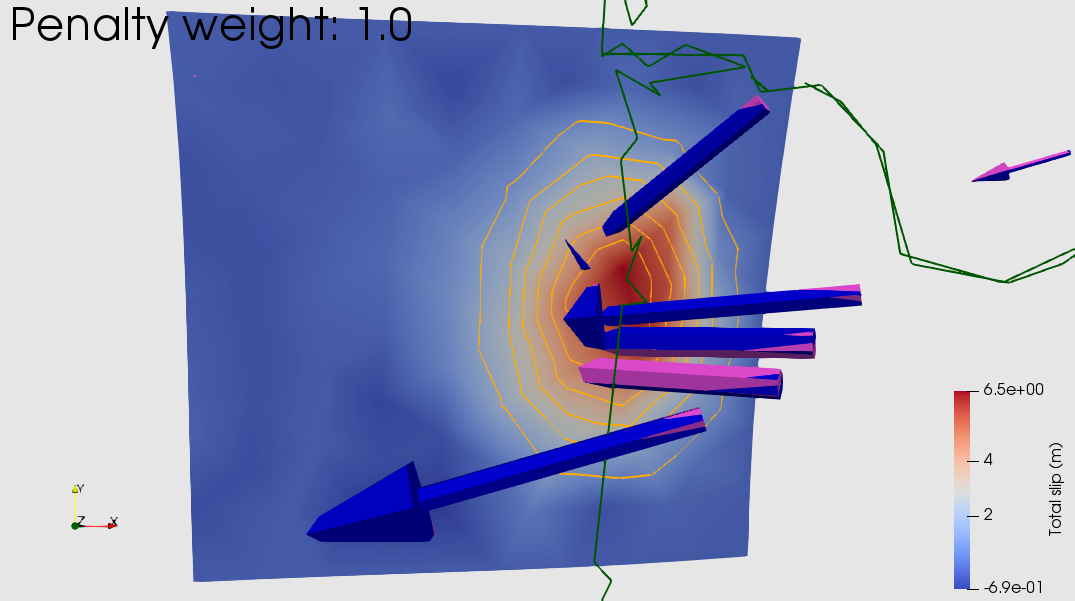
\includegraphics[width=4.5in]{examples/figs/subduction3d_step07_inverse_soln}
  \caption{ParaView image of the inversion solution for a penalty
    weight of 1.0. 'Data' is shown with blue arrows and predicted
    displacements are shown with magenta arrows. Color contours
    represent the predicted slip distribution and orange line contours
    show the applied slip from the forward problem.}
  \label{fig:example:subduction:3d:step07:invresults}
\end{figure}

\subsubsection{Exercises}

\begin{itemize}
\item Investigate the effects of data noise.
  \begin{itemize}
  \item How do the noisy data vectors compare to the raw data vectors
    from example step06?
  \item Create a new simulated dataset with more noise and see how
    well the solution matches the applied slip.
  \end{itemize}
\item Different initial slip distribution.
  \begin{itemize}
  \item Move the slip distribution to a different location, vary the
    amplitude, etc. This will involve running another instance of example
    step06 to create a new dataset. How is the solution affected?
  \item Move the slip onto the splay fault. This will involve creating
    a new forward model as well as generating Green's functions for the
    splay fault.
  \end{itemize}
\item What happens if your material properties are incorrect?
  \begin{itemize}
  \item Try creating your forward model with heterogeneous properties
    and your Green's functions with homogeneous properties (or
    vice-versa). What happens to your solution?
  \end{itemize}
\item Try inverting for slip at various time steps.
\item Try a different inversion method.
  \begin{itemize}
  \item If you analyze the predicted slip distribution you will find
    some negative slip, which is unrealistic. To overcome this problem
    you could try NNLS (non-negative least squares). If you have the
    scipy package installed on your computer, you could replace the
    generalized inverse solution with the NNLS package included in
    \filename{scipy.optimize.nnls}.
  \end{itemize}
\end{itemize}

% ----------------------------------------------------------------------
\subsection{Step 8: Stress Field Due to Gravitational Body Forces}

This example demonstrates the use of gravitational body forces in
PyLith simulations, as well as the use of initial stresses to balance
the body forces. We also demonstrate what happens when the initial
stresses are not in balance with the gravitational stresses, and show
how viscoelastic problems with gravitational stresses will in general
will not reach a steady-state solution. We do not include faults in
this example. The example is divided into three sub-problems:
\begin{itemize}
\item Step08a: Gravitational body forces with 3-D density variations
  in elastic materials and initial stresses for a uniform density.
\item Step08b: Gravitational body forces with 3-D density variations
  in elastic materials and initial stresses from Step08a (initial
  stresses satisfy equilibrium, so there is no deformation).
\item Step08c: Gravitational body forces with 3-D density variations
  in elastic and viscoelastic materials and initial stresses from
  Step08a plus finite strain formulation (does not reach a steady-state
  solution).
\end{itemize}

For the first sub-problem (step08a), we apply gravitational stresses
and attempt to balance these with analytically computed stresses
consistent with the density of the mantle. Since the densities are not
constant, the forces are out of balance and we end up with significant
deformation. We first apply gravity and set the simulation time to
zero (static problem):
\begin{cfg}
<h>[pylithapp.timedependent]</h>
# Set gravity field (default is None).
<f>gravity_field</f> = spatialdata.spatialdb.GravityField

<h>[pylithapp.problem.formulation.time_step]</h>
# Define the total time for the simulation.
<p>total_time</p> = 0.0*year
\end{cfg}
Then, for each material, we use the same spatial database for the
initial stresses. We use linear interpolation and in the database the
initial stress is simply computed as $\{rho}_mgh$, where $\{rho}_m$ is
the density of the mantle material and $h$ is the depth below the
ground surface:
\begin{cfg}
# We specify initial stresses for each material via a SimpleDB and linear interpolation.
<h>[pylithapp.problem.materials.slab]</h>
<f>db_initial_stress</f> = spatialdata.spatialdb.SimpleDB
<p>db_initial_stress.label</p> = Initial stress in the slab
<p>db_initial_stress.iohandler.filename</p> = spatialdb/mat_initial_stress_grav.spatialdb
<p>db_initial_stress.query_type</p> = linear

<h>[pylithapp.problem.materials.wedge]</h>
<f>db_initial_stress</f> = spatialdata.spatialdb.SimpleDB
<p>db_initial_stress.label</p> = Initial stress in the wedge
<p>db_initial_stress.iohandler.filename</p> = spatialdb/mat_initial_stress_grav.spatialdb
<p>db_initial_stress.query_type</p> = linear

<h>[pylithapp.problem.materials.mantle]</h>
<f>db_initial_stress</f> = spatialdata.spatialdb.SimpleDB
<p>db_initial_stress.label</p> = Initial stress in the mantle
<p>db_initial_stress.iohandler.filename</p> = spatialdb/mat_initial_stress_grav.spatialdb
<p>db_initial_stress.query_type</p> = linear

<h>[pylithapp.problem.materials.crust]</h>
<f>db_initial_stress</f> = spatialdata.spatialdb.SimpleDB
<p>db_initial_stress.label</p> = Initial stress in the crust
<p>db_initial_stress.iohandler.filename</p> = spatialdb/mat_initial_stress_grav.spatialdb
<p>db_initial_stress.query_type</p> = linear
\end{cfg}

The output parameters are simply the output filenames, since all the
other parameters are the defaults in \filename{pylithapp.cfg}. We use
the algebraic multigrid solver, which is appropriate for problems with
no fault. We run the sub-problem by doing:
\begin{shell}
$$ pylith step08a.cfg mat_elastic.cfg solver_algebraicmultigrid.cfg
\end{shell}

When the problem has run, we see deformation that is consistent with
the mismatched densities. Figure
\vref{fig:example:subduction:3d:step08a} demonstrates the deformed
mesh visualized by running the following command from the
\filename{subduction} directory:
\begin{shell}
./viz/plot_dispwarp.py --sim=step08a --exaggeration=500.0
--screenshot=subduction3d_step08a_soln.png
\end{shell}
\begin{figure}
  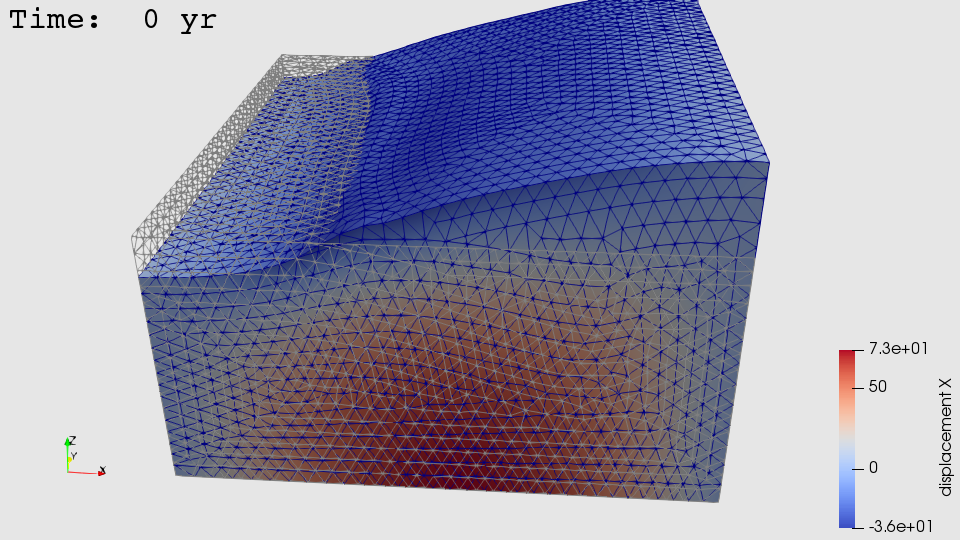
\includegraphics[width=4.5in]{examples/figs/subduction3d_step08a_soln}
  \caption{Image generated by running the \filename{plot\_dispwarp.py}
    script for sub-problem step08a. The crustal material to the
    east is lighter than the assumed mantle material for initial
    stresses, while the slab material to the west is heavier. The
    result is uplift to the east and downward movement to the west.}
  \label{fig:example:subduction:3d:step08a}
\end{figure}

% End of file
